\documentclass[12pt]{elsarticle}
\usepackage{setspace}
\doublespacing

\usepackage{graphicx}
\usepackage{amssymb}
\usepackage{lineno}
\setlength\parindent{0pt}
\usepackage{multirow}
\usepackage{tabularx,ragged2e}
\newcolumntype{C}{>{\Centering\arraybackslash}X} % centered "X" column
\usepackage{float}
\usepackage{graphicx}
\usepackage{pdflscape}
\usepackage[center]{caption}
\usepackage[super]{nth}
\usepackage{minted} %for python
\usepackage{listings}
\usepackage{hyperref}
\usepackage{comment}
\usepackage{bookmark}
\usepackage{titlesec}
\usepackage{amsmath}

\usepackage{natbib}
\bibliographystyle{agsm}

\newcommand{\sectionbreak}{\clearpage}

\usepackage{graphicx}
\usepackage{subfig}

\graphicspath{ {./images/} {./graphs/} }

\makeatletter
\def\ps@pprintTitle{%
\let\@oddhead\@empty
\let\@evenhead\@empty
\def\@oddfoot{\centerline{\thepage}}%
\let\@evenfoot\@oddfoot}
\makeatother

\begin{document}

\begin{frontmatter}

\title{Movie Recommendation System}

\author{Tiberiu Simion Voicu}

\address{Post graduate thesis project, ECS751P}

\begin{abstract}
    Recommender systems aim to provide users with personalized recommendations of items. This helps a lot in filtering irrelevant items from the big collection. It is usually achieved through collaborative filtering. 
    Neural networks have proven to be highly effective in natural language processing, computer vision and speech recognition. Despite this, they haven't seen as much use in solving recommendation problems. This is partly because state of the art matrix factorization methods are already very effective for this problem. The system described in this paper will make use of multilayer perceptron networks to solve the recommendation problem using collaborative filtering. The design and implementation details of the recommendation engine will be discussed and the results compared with traditional matrix factorization methods. Furthermore, it will also go into detail about the choices that went into creating a scalable overall system and accompanying web application.
\end{abstract}

\end{frontmatter}

\newpage
\tableofcontents

\section{Introduction}
Nowadays every customer is faced with a multitude of possible choices. Because of this, it is very important that the user doesn't have to waste time manually filtering through the items to find relevant ones. Recommender systems overcome this by providing personalized recommendations that suit a particular users' tastes. They are present in many different websites such as google, amazon, and netflix and help highly with user retention and satisfaction. I will focus on the problem of recommending movies and also building the underlying system and infrastructure required to serve these recommendations.

\subsection{Dataset}
The dataset used as the basis for the recommendation engine is the movie lens 20m dataset, put together by the Grouplens research group at the University of Minnesota \citet{movielens}.
This is an explicit feedback dataset, where users manually assigned ratings to movies. The characteristics of this dataset are the following.
\begin{itemize}
    \item 20000263 ratings on a scale of 0.5-5 in 0.5 increments
    \item 27278 movies having been rated at least once
    \item 138493 users that have rated at least 20 movies
    \item 465564 tags about movies
\end{itemize}
The dataset is split into different files of which I am only using the ratings, movies and links files. 
They are all available in comma-separated value format.
The ratings file comprises of values for userId, movieId, rating, and timestamp.\ref{ratingsFile}. Timestamp remains unused while the other values are used together to perform collaborative filtering.
The movies file is made up of movieId, title, and genre. \ref{moviesFile} It is used for incorporating genre data into the model.
The links file contains movieId, imdbId and tmdbId. \ref{linksFile} This file provides imdbId and tmdbId used in web-scraping scripts to provide content for the demo web-app.

\begin{center}
    \begin{tabular}{||c c c c||} 
    \hline
    userId & movieId & rating & timestamp \\ [0.5ex] 
    \hline\hline
    57772 & 3861 & 4.0 & 982690041 \\ 
    \hline
    122521 & 1411 & 2.0 & 1001957487 \\
    \hline
    22759 & 46578 & 4.0 & 1216540196 \\
    \hline
    92812 & 1206 & 2.5 & 1118792437 \\ [1ex] 
    \hline
   \end{tabular}
\captionof{table}{Rating file}\label{ratingsFile}
\end{center}

\begin{center}
    \begin{tabular}{||c c c||} 
    \hline
    movieId & title & genres \\ [0.5ex] 
    \hline\hline
    106749 & Mr. Morgan's Last Love (2013) & Comedy\textbar Drama \\ 
    \hline
    2 & Jumanji (1995) & Adventure\textbar Children\textbar Fantasy\\
    \hline
    91169 & Easier with Practice (2009) & Drama\textbar Romance \\
    \hline
    106879 & Fright Night 2: New Blood (2013) & Horror \\ [1ex] 
    \hline
   \end{tabular}
\captionof{table}{Movie file}\label{moviesFile}
\end{center}

\begin{center}
    \begin{tabular}{||c c c||} 
    \hline
    movieId & imdbId & tmdbId \\ [0.5ex] 
    \hline\hline
    6 & 0113277 & 949 \\ 
    \hline
    206 & 0114805 & 77350 \\
    \hline
    71466 & 1174730 & 28053 \\
    \hline
    96834 & 2343601 & 111174 \\ [1ex] 
    \hline
   \end{tabular}
\captionof{table}{Links file}\label{linksFile}
\end{center}


\section{Background \& Related Work}
The most common types of recommender systems can be split into collaborative filtering and content based. They can be further split into model-based, and memory-based.

\subsection{Content Based}
Content based recommendations require several features related to an item instead of historic user-item interactions. In the case of movie recommendations, these could be year, actors, genres, producers, writers, etc.
This method relies on calculating the similarity between items using features such as the ones previously stated.
The general idea is that if a user likes a given item he will also like items similar to it. One way of achieving this is by calculating term frequency (TF) and inverse document frequency (IDF) of the items. Then using the vector space model and a choice of similarity metrics such as cosine or pearson, we can compare different items \citet{MF_Techniques}.
Another way of achieving this is to represent different content items as dense vectors that can be easily fed into a neural network architecture.

\subsection{Collaborative Filtering}
Collaborative filtering (CF) algorithms aim to recommend items to a user by combining the item interactions of a given user with item interactions of all other users. CF can be split into two categories. User-based where the aim is to measure the similarity of a given user and all other users. Item-based where we aim to measure the similarity between the items a given user has interacted with and other items.
The most widely used method of achieving this is through factorization of the very sparse user-item interaction matrix.

\subsection{Matrix Factorization}
The idea behind matrix factorization (MF) is to decompose the matrix R containing user-item interactions, into the product of two lower dimensional matrices P of size \(n X k\) and Q of size \(k X m\). Matrix P is the user matrix where n is the number of users, k the number of latent factors and \(p_u\) is the latent vector of user u. The other matrix is the movie matrix with m number of movies, the same k latent factors and \(q_i\) is the latent vector of item i. The predicted rating \(\hat{y}_{ui}\) can then be calculated by taking the dot product of those two vectors \citet{MF_Techniques}.

\begin{equation}
    \hat{y}_{ui} = f(u,i|P_{u}Q_{i}) = P_{u}^{T}Q_{i} = \sum_{K=0}^{k}P_{uk}Q_{ik}
\end{equation}

Singular value decomposition (SVD) and non-negative matrix factorization (NMF) are two techniques successfully applied in literature to achieve the decomposition.
SVD is the general case for principal component analysis

The resulting matrices are dense and have much lower dimension than the initial matrix R. By choosing a different number of latent factors we can include more or less abstract information about the initial matrix R. MF poses the recommendation problem as a regression optimization one. Two common metrics used for this are root mean squared error (RMSE) and mean absolute error (MAE). The RMSE and MAE can be calculated as follows given that, \(e_i\) is the difference between the actual and predicted value of rating i. 
\begin{equation}
    RMSE = \sqrt{\frac{1}{n}\sum_{i=1}^{n}{e^2_i}}
\end{equation}
\begin{equation}
    MAE = \frac{1}{n}\sum_{i=1}^{n}{\mid e_i\mid}
\end{equation}

Stochastic gradient descent (SGD) and alternating least square (ALS) are two optimization algorithm generally employed to learn a good approximation.

\begin{itemize}
    \item Set item factor matrix constant and adjust user factor matrix by taking the cost function derivative.
    \item Set user factor matrix constant and adjust item factor matrix.
    \item Repeat until convergence.
\end{itemize}

\subsection{Neural Networks \& Deep Learning}
Neural networks are universal approximators, typically organized in layers of neurons connected through weights and put through an activation function. The number of layers and neurons at each layer also called the depth and width of the network are variable and many different configurations seem to work in practice. The simplest neural network is made up of 3 layers, input, hidden and output.

\begin{figure}[h!]
    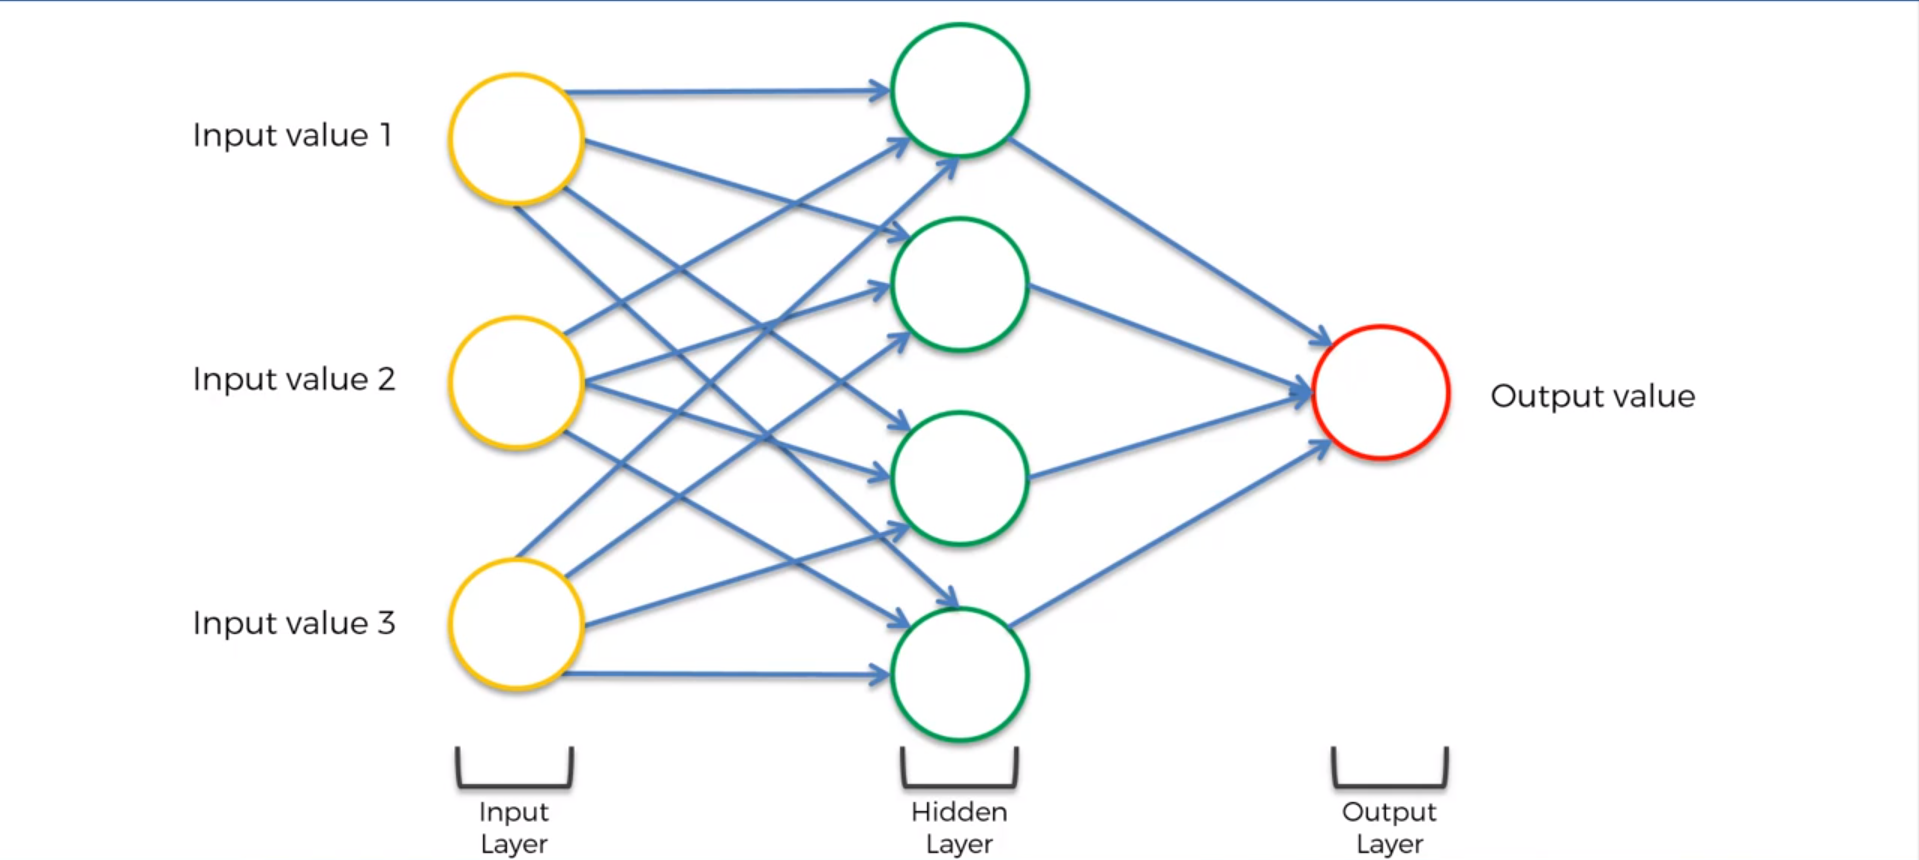
\includegraphics[scale=0.2]{nn-3-layers}
    \caption{3 Layer Neural Network}
\end{figure}

They can be used for both supervised and unsupervised learning and can be applied to classification and regression problems just as effectively. Deep neural networks (DNN) are NN of more than 3 layers, although in practice and state of the art implementations these are many layers deep and very wide as well. The main benefit of using NNs algorithms is that they don't require manual feature engineering.
A big disadvantage is the lack of interpretability for the predictions, due to this NN are generally viewed as black boxes. This means that we are not aware of the `why` and `how` did the network product a certain output given some inputs. This could be especially detrimental in the context of recommendation systems because the users might wish to know the reasons behind their recommendations. Other memory and similarity based methods provide much more transparency in this regard.

Different classes of NN have emerged in literature including convolutional networks (CNN), autoencoders (AE), recurrent networks (RNN), generative adversarial networks (GAN) besides of simple fully connected multilayer perceptrons (MLP).

\subsection{Related Work}
\citet{HybridAutoencoders} propose a hybrid recommender system based on auto-encoders
\citet{NeuralCF} propose a neural collaborative filtering system using implicit training data for training.


\section{System Architecture}
\subsection{Technologies, tools and frameworks}
\subsubsection{React}
React is a fast, declarative and efficient javascript library for creating web interfaces. It works around the concept of components. They are self-contained and composable blocks of code that encapsulates a part of user interface and its functionality. By putting together multiple small components it's possible to build complex user interfaces (UI). Components can be stateful or stateless.
The library provides a virtual-dom similar to the browsers document object model (DOM). They are both node trees that list elements together with attributes and content as objects and properties. Updating the dom is rather slow which is why the virtual-dom is useful for efficiency. It allows react to optimize DOM updates under the hood to only happen when it's necessary.
\subsubsection{Docker \& Containers}
Containers are self contained pieces of code that can be run on any computer and operating system (OS). They contain the code and all of its necessary parts such as libraries, tools and frameworks. They are similar to virtual machines but the main difference is in efficiency and application size. Containers are more efficient and smaller because they run on the same underlying kernel as the operating system as as opposed to virtual machines which runs an entirely different OS.

Docker is tool that allows creating and running containers and managing containers. 
Docker

\begin{figure}[h!]
    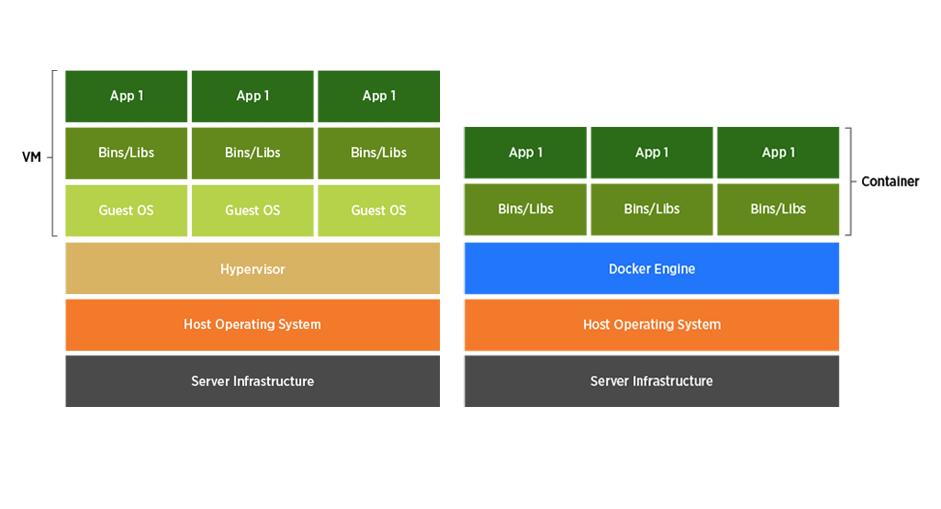
\includegraphics[scale=0.5]{containers-vs-vm-diagram}
    \caption{Containers and virtual-machine comparison diagram}
\end{figure}

\subsubsection{Kubernetes}
Kubernetes is a container orchestration platform created by google and open sourced in 2014. It allows automation of deployment, scaling and management of containerized applications. It groups the container that make up a multi micro-service application into logical units for easy discovery and management. It's built with scalability in mind 

Node 
Pod
Service
Gateway
Ingress

\subsubsection{Mongodb \& Mongoose}

\subsection{Micro-services}
Authentication

Gateway

User

Search

Engine

\begin{figure}[h!]
    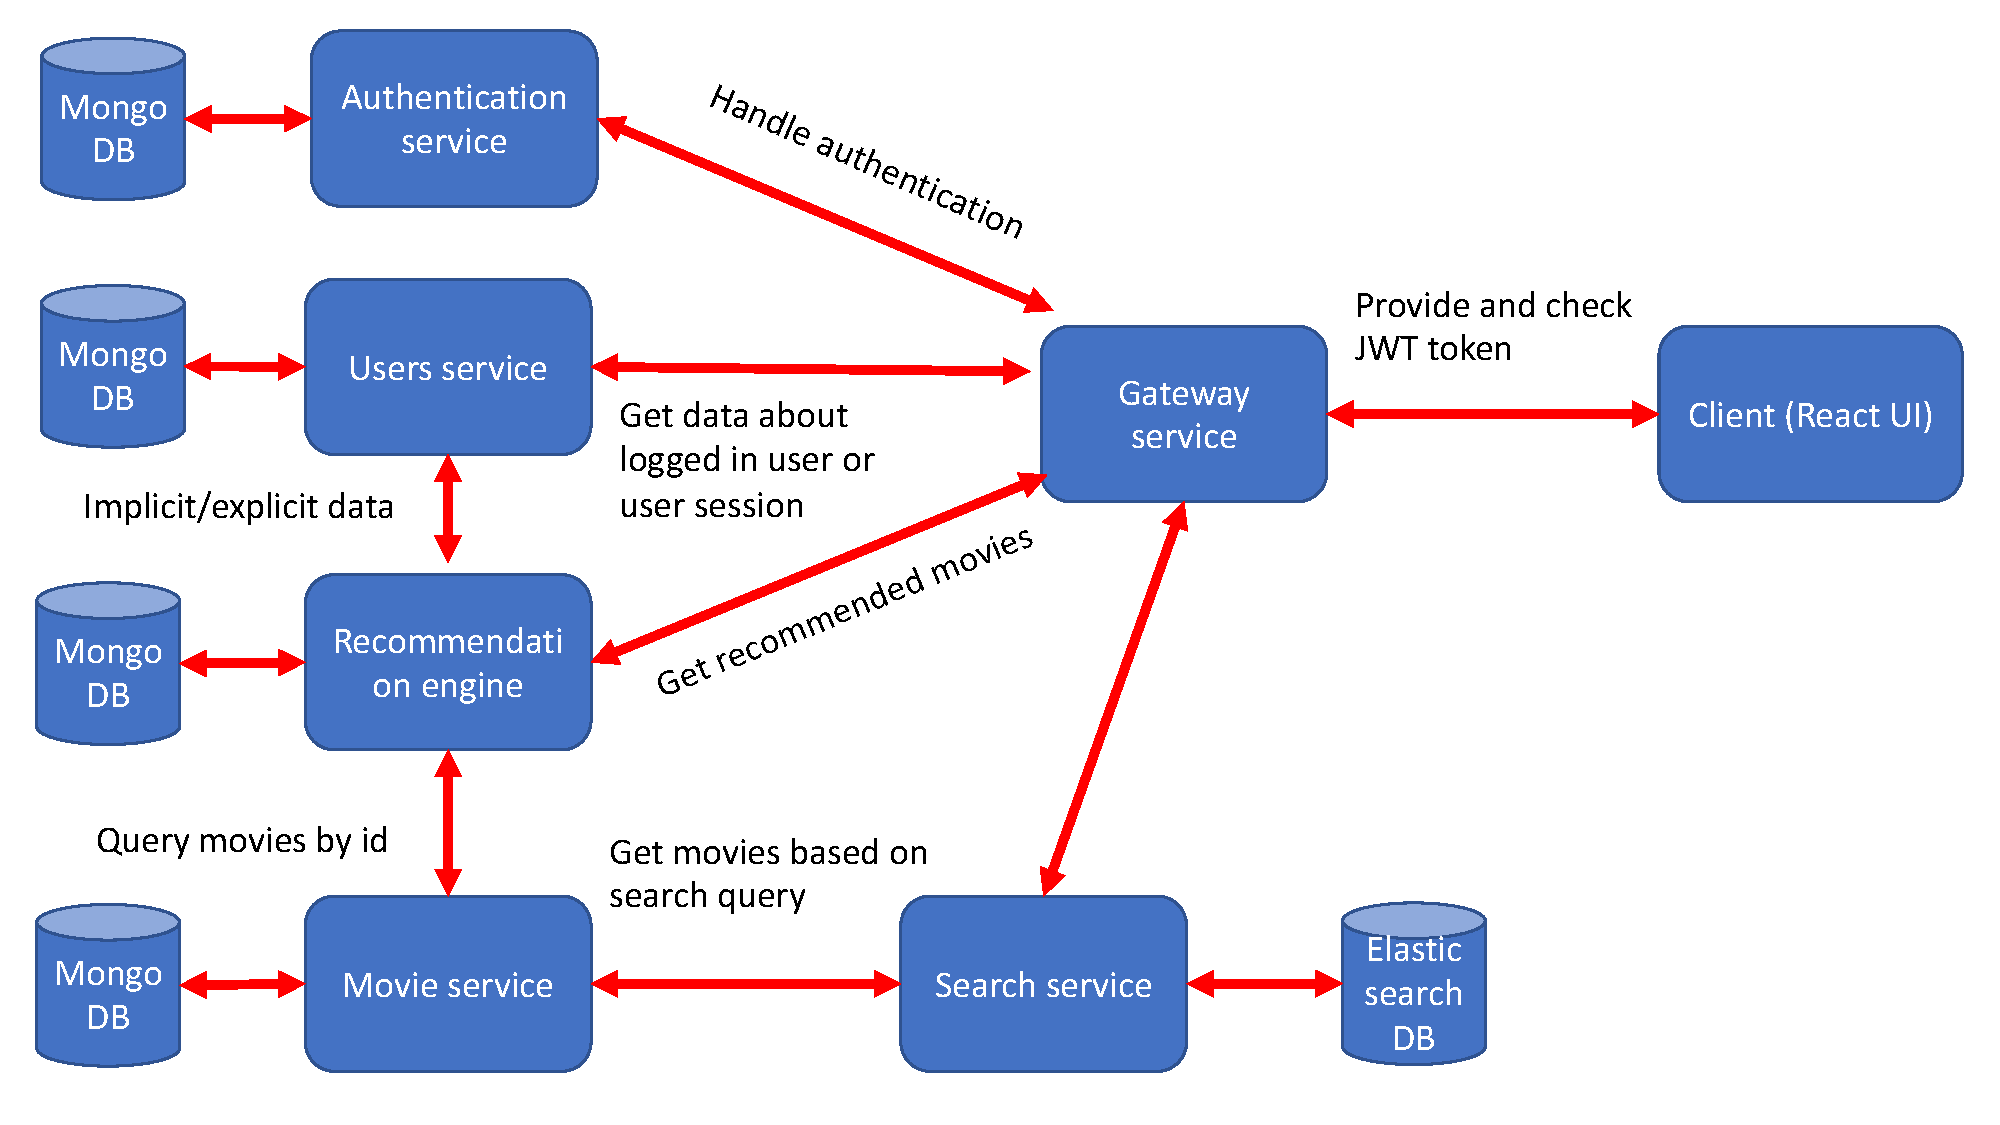
\includegraphics[scale=0.4]{architecture_diagram}
    \caption{Architecture diagram}
\end{figure}

\begin{figure}[h!]
    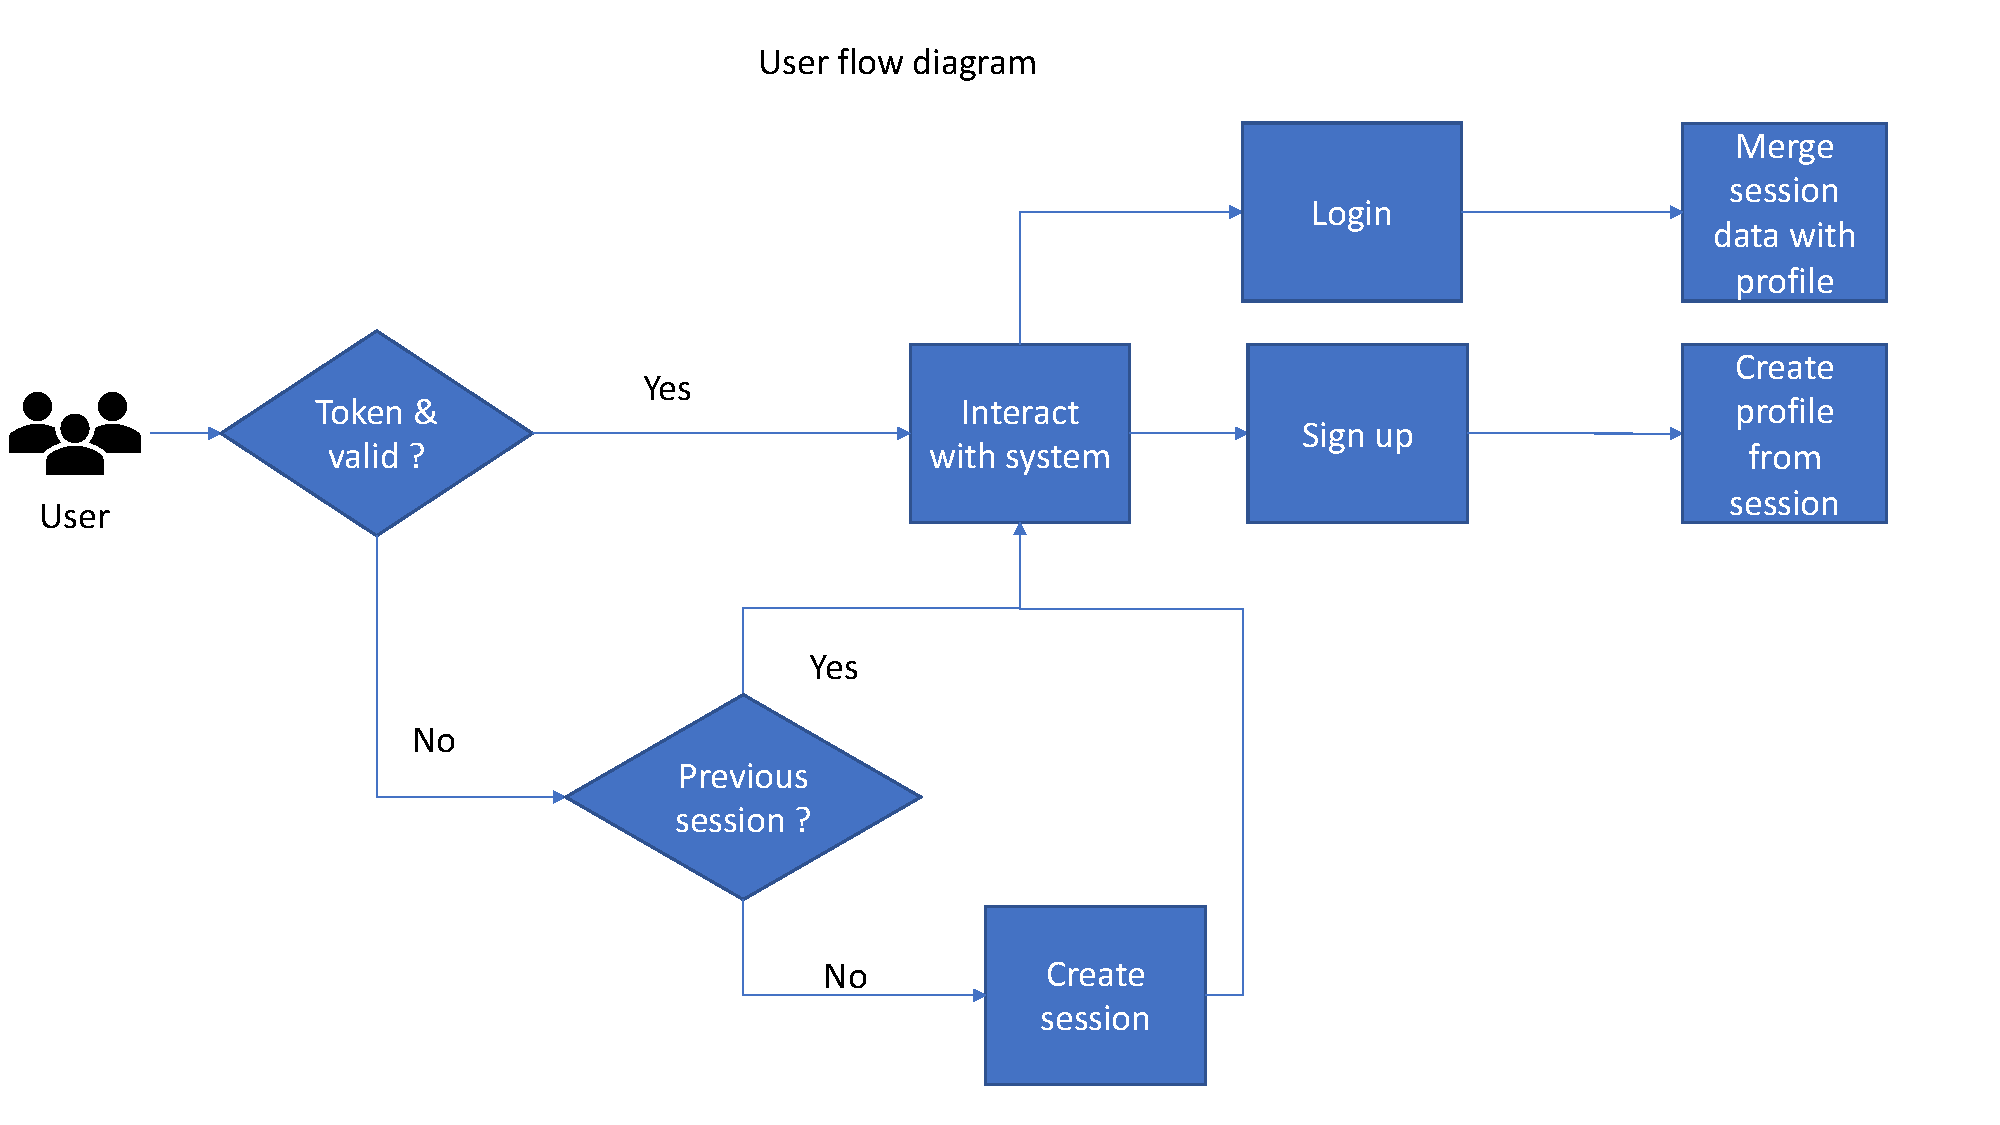
\includegraphics[scale=0.4]{user_flow_diagram}
    \caption{User flow diagram}
\end{figure}

% \subsection{Database}
\subsection{Web application}


\section{Recommendation Engine}

\subsection{Embeddings}
Neural networks do not deal well with categorical variables. One hot encoding is a way to handle this. It allows us to represent categorical data as sparse vectors of zeroes and a single 1 representing the specific category. This method has two main drawbacks. Firstly, the dimensionality of the vector representation size grows with the corpus. It can become unmanageable very quick. Secondly, each vector is equidistant from every other vector. This means 'similar' categories are not represented close together in the vector space.

A better way of handling categorical data is through embeddings. When using embeddings we can project categories in a low dimensional latent space and represent them as dense continuous vectors. They are learned parameters and due to this, similar items are projected close together in the latent space. Therefore it is useful in the context of recommendations as we are trying to model user-item similarities. They are also well studied and highly applied in literature for natural language processing to represent words (\citet{embeddings}). Embeddings can be pre-trained and adapted to be used in a model or learned end-to-end with the other parameters.

The main inputs to the model consist of user, item and genre embeddings learned iteratively with the rest of the model parameters.

Genres are handled slightly different than the other two because a movie can have more than one genre. The basis of the embedding is a multi hot encoding, meaning the vector has a value of one for each category that describes it.

\subsection{Activation function}
In a neural network activation functions are mathematical equations, applied to each neuron, that determine if it should activate or not based on its inputs. This function must be computationally efficient to calculate, differentiable and will generally be non-linear. The last part is very important because without non-linearities a NN would just behave like a single-layer perceptron and would not be able to model complex functions. One exception to this is the output layer for a regression NN which will have a linear activation to allow the prediction of any real value.

Early neural networks were using hyperbolic tangent (tanH) and sigmoid activation functions. Sigmoid also known as logistic function is S-shaped and bounded by 1 and 0 \ref{eq:sigmoid}. It suffers from vanishing gradient for very high or low values of x which can result in the network refusing to learn after some point. TanH function is similar to sigmoid but suffers less from the vanishing gradients problem \ref{eq:tanh}.
\begin{equation}
    \label{eq:sigmoid}
    \begin{aligned}
    f(x) &= \frac{1}{1+e^{-x}} \\
    f'(x) &= f(x)(1 - f(x))
    \end{aligned}
\end{equation}

\begin{equation}
    \label{eq:tanh}
    \begin{aligned}
    f(x) &= \frac{2}{1+e^{-2x}} - 1 \\
    f'(x) &= 1 - f(x)^2
    \end{aligned}
\end{equation}

Rectified Linear Unit (ReLU) was first introduced by \citet{relu} in 2010 and is nowadays highly used in deep learning. It introduces sparsity in the network because it outputs 0 for negative numbers \ref{eq:relu}. Moreover, reLU is more computationally efficient than the other two activations. However, a major drawback of using ReLU activations is the "dying ReLU" problem. A ReLU is said to be 'dying' when its stuck outputting 0. The leakyReLU \ref{eq:leakyrelu} is an adaptation of the original. It allows a small value as output for negative samples. This fixes the problem of "dying ReLU" leading to a more robust model (\citet{leakyrelu}).

\begin{equation}
    \label{eq:relu}
    \begin{aligned}
    f(x) &=
    \begin{cases}
        x, & \text{if } x\geq 0 \\
        0, & \text{otherwise}
    \end{cases} \\
    f'(x) &=
    \begin{cases}
        1, & \text{if } x\geq 1 \\
        0, & \text{otherwise}
    \end{cases}
    \end{aligned}
\end{equation}

\begin{equation}
    \label{eq:leakyrelu}
    \begin{aligned}
    f(x) &=
    \begin{cases}
        x, & \text{if } x\geq 0 \\
        0.01x, & \text{otherwise}
    \end{cases} \\
    f'(x) &=
    \begin{cases}
        1, & \text{if } x\geq 1 \\
        0.01, & \text{otherwise}
    \end{cases}
    \end{aligned}
\end{equation}

\begin{figure}[h!]
    \subfloat[Activation functions]{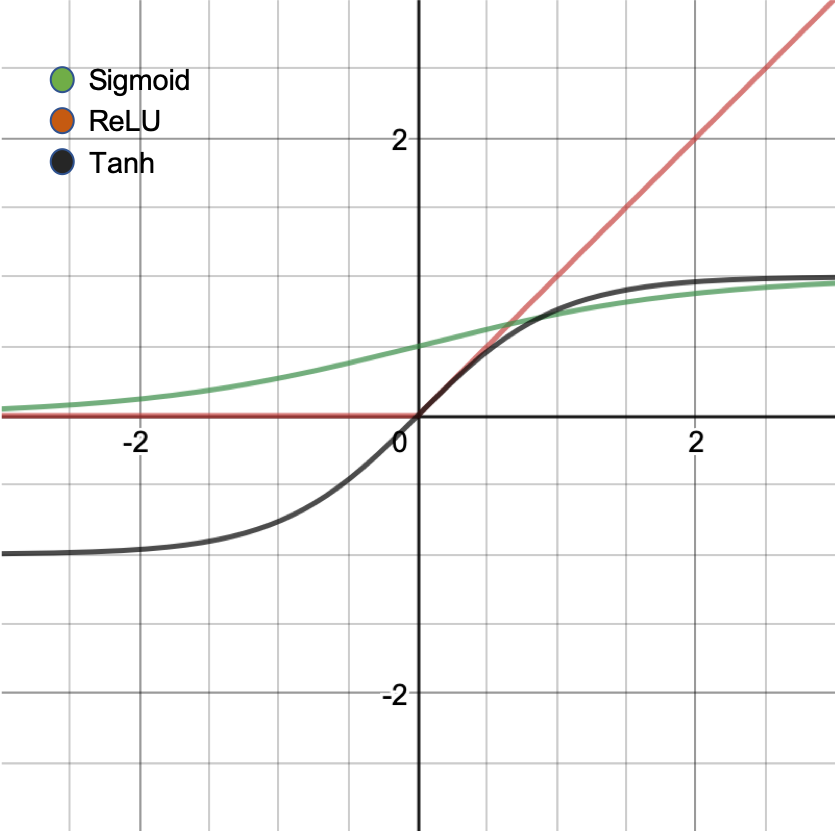
\includegraphics[scale=0.5]{3-activation-func}\label{fig:activations}}
    \hfill
    \subfloat[ReLU vs Leaky ReLU]{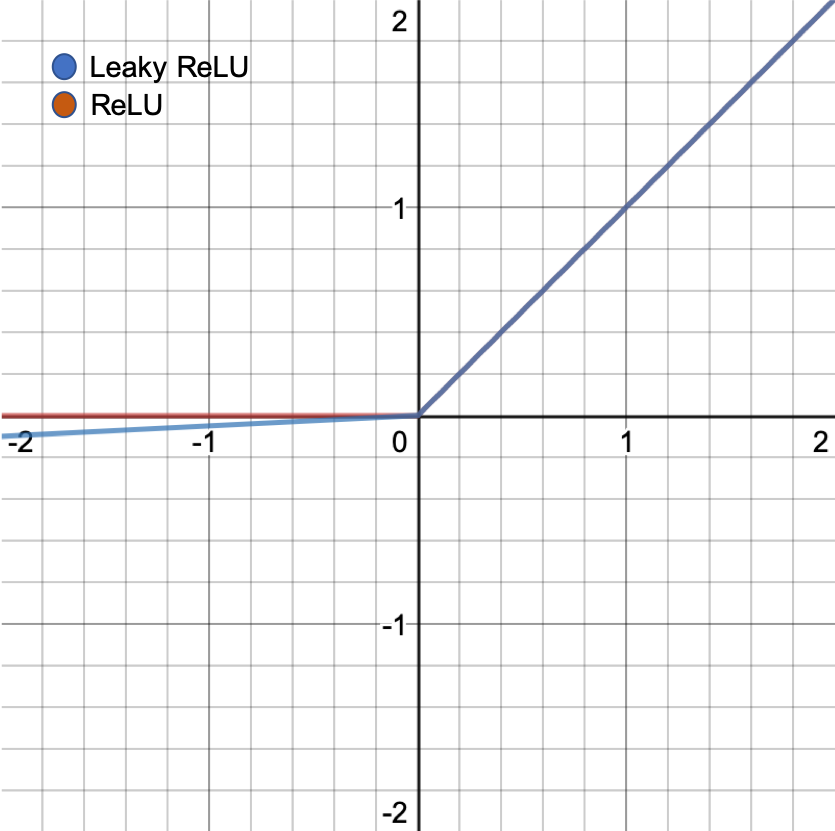
\includegraphics[scale=0.5]{leakyReLUvsReLU}\label{fig:relus}}
\end{figure}


\subsection{Regularization}
One of the most common problems in training neural networks is over-fitting. A model is said to be over-fitting when it performs well on training data but poorly on validation data. Intuitively, it means the model is unable to generalize well and only memorizes the training examples.
This generally occurs if the model is too complex or the size of the training dataset is too small.
Regularization is a method of reducing over-fitting through small modifications of the learning algorithm. The most common types of regularization are l1 and l2. L1 regularization adds the absolute value of the coefficients as penalty term to the cost function. This leads feature sparsity, which is desireable in some cases. L2 is similar but adds the squared value of coefficients as penalty term to the cost function. 

\begin{equation}
    \label{eq:l1l2}
    \begin{aligned}
    l1 penalty = \frac{\lambda}{2m} * \sum{\mid\mid w \mid\mid} \\
    l2 penalty =  \frac{\lambda}{2m} * \sum{\mid\mid w \mid\mid^2}
    \end{aligned}
\end{equation}

In the equations lambda is the hyperparameter controlling the regularization strength. The parameter is usually found using cross-validation or through experimentation. I have experimented with values between \(1e^{-4}\) and \(1e^{-8}\). The final model uses l2 weight regularization on embedding and dense layers with lambda of value \(1e^{-7}\).

Dropout is a special way to regularize the network. This changes the normal training routine by dropping random neurons with a probability p. The edges of a dropped neuron are also removed for that epoch. Therefore, at each epoch we train on a smaller model.
This stops the NN from depending too much on any specific neurons (\citet{dropout}). During testing or prediction phase dropout is disabled. The probability p of dropping neurons is another hyperparameter that has to be selected similar to $\lambda$ in l1 and l2. I have tried values of p between 0.1 - 0.5 in 0.1 increments. The best values of 0.2 and 0.5 are applied in the final model on embedding and dense layers respectively.

\subsection{Optimizer}
Optimizers are a very important parameter in NN configuration. Nowadays there is a vast choice of good optimizers. At its core, an optimizer is an iterative method of optimizing for a cost function. At each optimization step, the weights in the NN will be updated based on the negative of the gradient of the cost function. Stochastic gradient descent (SGD) is a variation of gradient descent in that the optimization happens after each training example. In practice, this usually implies mini-batches of between 32 and 1024 data points (\citet{practical_training}). Batch gradient descent involves updating the weights based on the gradient over the whole dataset. SGD optimizes based on an approximation of the gradient, unlike batch gradient descent. This turns out to be useful as it introduces noise in the network which leads to better generalization. It is also more scalable as the whole dataset does not have to be kept in memory. (\citet{practical_training})

\begin{equation}
    \theta = \theta - \alpha \Delta_{\theta} J(\theta ;x^{(i)}y^{(i)})
\end{equation}

More advanced optimizers are built on top of SGD and include things such as adaptive learning rates and momentum to increase convergence speed and overall stability.

One such algorithm is adaptive moment estimation (Adam). Its widely used in literature and converges much faster than SGD. Adam can be seen as a combination of RMSProp and momentum (\citet{Adam}). Adam uses estimations of first and second order moments of the gradient to adapt the learning rate for each weights in the network.

Nesterov adaptive moment estimation (NAdam) combines adam with nesterov momentum which improve convergence (\citet{NADAM}).

I have decided to use NAdam for training following experiments that proved its the best choice for this specific problem and on this dataset. I am using it with learning rate of $2e^{-4}$, epsilon value of $1e^{-4}$, and the other parameters are keras defaults for this optimizer.

\subsection{Training}
Weight initialization plays an important role in training a neural network. Ideally, we wish the initial weights to be random but not too small and too big, otherwise, it will lead to problems of vanishing or exploding gradients. Xavier normal initialization is one technique that constricts the weights to these characteristics. It works by drawing from a truncated random distribution centered on 0 and with a standard deviation of \(\frac{2}{n_{in} + n_{out}}\), where \(n_{in}\) and \(n_out\) represent the number of inputs and outputs (\citet{initialization}). This is the default initializer used in keras. It is best suited for use in NN that employ tanh activation functions. He normal initialization works better for relu activation. Its similar to xavier, but the standard deviation is \(\frac{2}{n_{in}}\) (\citet{rectifiers}).

\begin{verbatim}
    xavier_w = np.random.rand((n_in, n_out)) * np.sqrt(2 / (n_in + n_out))
    he_w = np.random.rand((n_in, n_out)) * np.sqrt(2 / n_in)
\end{verbatim}

Too speed up the training I have implemented a special generator class extending keras \emph{sequence}. This enables multiprocessing execution of the batch generation algorithm and more importantly it ensures safety and single use of each training example per epoch.
After creating the generator its possible to use the keras \emph{fit\_generator} function with the number of workers and max processing queue size instead of \emph{fit}. This achieves a good speed up in training as the GPU does not have to wait for the CPU to prepare the training batch. More importantly, with these changes it's possible to train on multiple GPUs using data parallelization. In this case the batch will be divided equally among the GPUs. 
Moreover, I have enabled the keras callback \emph{EarlyStopping} with patience of six. This acts as regularization method, because it stop training after the model validation loss has not decreased for 6 consecutive epochs. Moreover, it also rewinds the model parameters to the epoch that had the best loss.

Batch Normalization is a technique proposed by \citet{batchnorm}, which aims to reduce the amount by which hidden unit values shift. It normalizes the input to a layer by subtracting the batch mean and dividing by the batch standard deviation. It turns out this leads to faster convergence and more stability in training. Furthermore, the batch normalization layers also have a small regularization effect which helps the network generalize better.

Finally, the model was trained using 12 workers, a queue size of 200, and batch of 512 data points split evenly between 4 GPUs.

\subsection{Architecture}
The NN architecture follows a common tower pattern, where layers near the top are widest and progressively decrease in width. The inputs to the network consist of user, movie and genre embeddings and average movie and user ratings. They are then concatenated fed into the first hidden layer.
The activation functions employed at the hidden layers are leakyReLU. Each hidden and embedding layer is followed by a dropout layer and a batch normalization layer. The output is made up of a single neuron with linear activation. 

\begin{figure}[h!]
    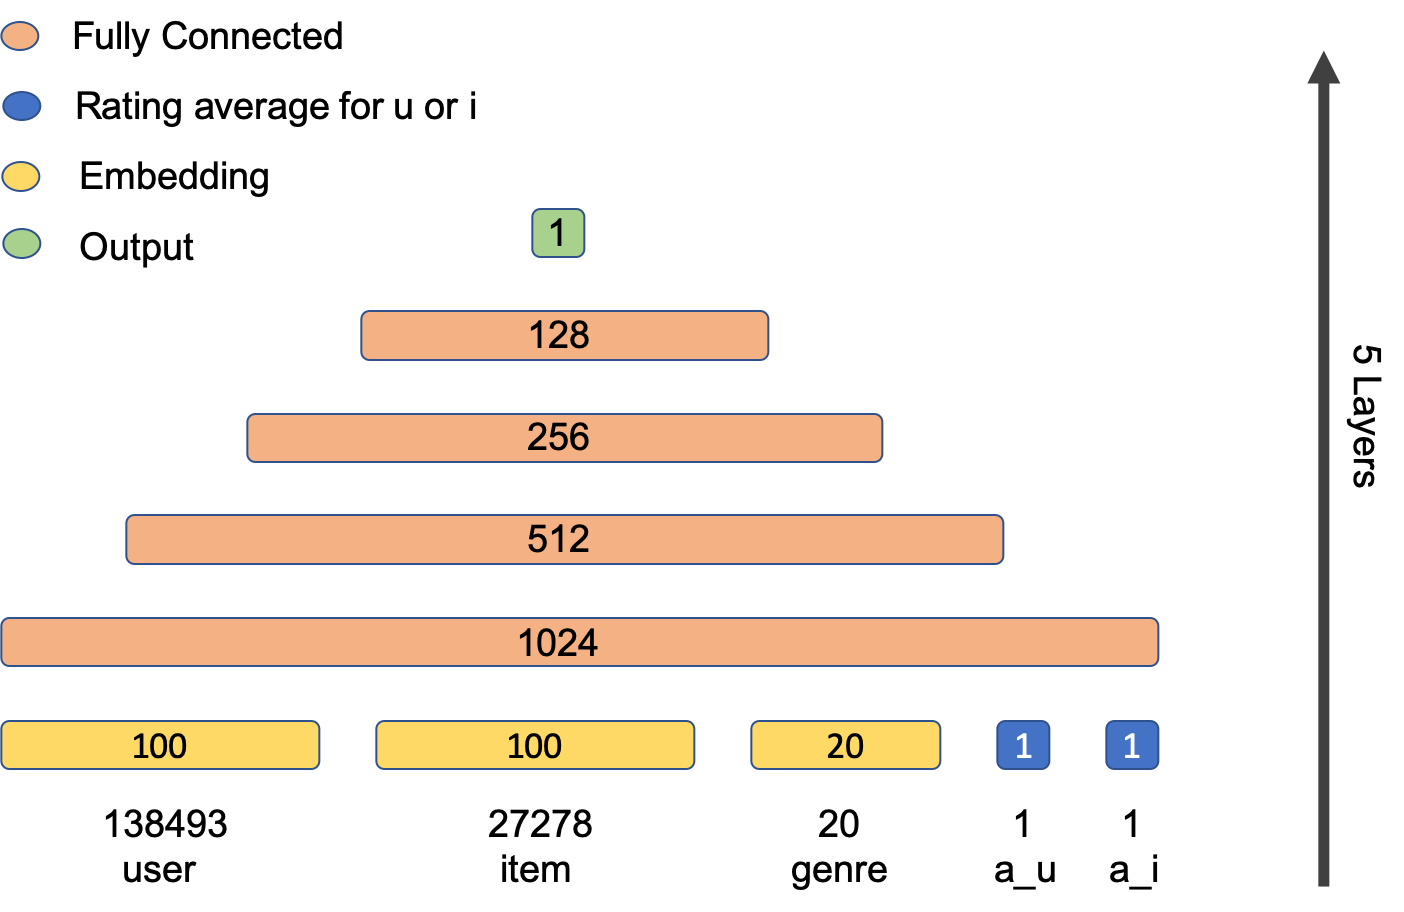
\includegraphics[scale=0.6]{nn_architecture.png}
    \caption{Network architecture}
\end{figure}

\section{Evaluation}
The evaluation section with results

\begin{figure}[h!]
    \subfloat[RMSE plot]{\includegraphics[scale=0.5]{RMSE}\label{fig:RMSE}}
    \hfill
    \subfloat[MAE plot]{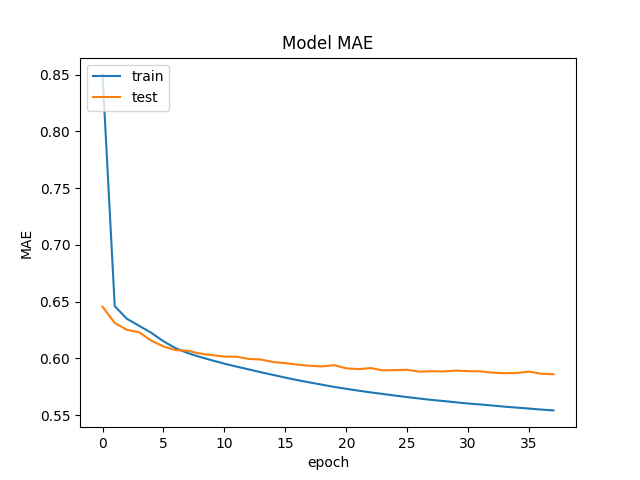
\includegraphics[scale=0.5]{MAE}\label{fig:MAE}}
\end{figure}

\begin{center}
    \begin{tabular}{||c c c||} 
    \hline
    Model & RMSE & MAE \\ [0.5ex] 
    \hline
    SVD & 0.8152 & 0.6190 \\ 
    \hline
    NMF & 0.8246 & 0.62876 \\
    \hline
    NNCF+genres & 0.7763 & 0.5861 \\ [1ex]
    \hline
   \end{tabular}
\captionof{table}{Results Comparison (RMSE \& MAE)}\label{comparison}
\end{center}

\section{Conclusion}
\subsection{Future Work}
Possible improvements to the system include the following.
\begin{itemize}
    \item Incorporate more content information into the system such as movie title, summary, and cast. This could be achieved using pre-trained word embeddings such as word2Vec or glove.
    \item Add recurrent layers such as GRU or LSTM.
    \item Train a convolutional network on movie posters. Then incorporate said network into the CF model.
\end{itemize}

\bibliography{bibliography}
\newpage
\appendix
\begin{lstlisting}[language=Python]
    class Generator(Sequence):
        def __init__(self, data, user_avg_ratings, movie_avg_ratings, batch_size):
            self.data = data
            self.user_avg_ratings = user_avg_ratings
            self.movie_avg_ratings = movie_avg_ratings
            self.batch_size = batch_size

        def __len__(self):
            return int(np.floor(len(self.data) / float(self.batch_size)))

        def __getitem__(self, idx):
            batch = self.data.take(np.arange(idx * self.batch_size, (idx + 1) * self.batch_size, 1), 0)
            userIds = batch.loc[:]['userEmbeddingId'].values
            movieIds = batch.loc[:]['movieEmbeddingId'].values
            genreEmbeddings = np.array(list(map(lambda x: np.array(x), batch.loc[:]['genreEmbedding'].values)))
            ratings = batch.loc[:]['rating'].values

            userAvgRatings = np.array([self.user_avg_ratings.get(i) for i in userIds.tolist()])
            movieAvgRatings = np.array([self.movie_avg_ratings.get(i) for i in movieIds.tolist()])

            # return [[userIds, movieIds, genreEmbeddings], ratings]
            return [[userIds, userAvgRatings, movieIds, movieAvgRatings, genreEmbeddings], ratings]
\end{lstlisting}

\end{document}
